\section{Technical Background}
\label{app:technical_background}
\subsection{Group Relative Policy Optimization (GRPO)}

GRPO \cite{Shao2024DeepSeekMathPT} is a reinforcement learning algorithm designed for training language models with group-based advantage estimation. For each question $q$, a group of outputs $\{o_1, o_2, \cdots, o_G\}$ are sampled from the old policy model $\pi_{\theta_{old}}$. and optimizes the current policy $\pi_{\theta}$ using:

\begin{equation}
\begin{aligned}
\mathcal{J}_{\mathrm{GRPO}}(\theta)
=
\mathbb{E}_{q \sim P(Q),\, \{o_i\}_{i=1}^{G} \sim \pi_{\theta_{\mathrm{old}}}(\cdot \mid q)}
\\
\frac{1}{G}
\sum_{i=1}^{G}
\frac{1}{|o_i|}
\sum_{t=1}^{|o_i|}
\Big(
\min \Big[
r_{i,t}(\theta)\,\hat{A}_{i,t},\,
\\
\mathrm{clip}\!\left(
r_{i,t}(\theta),\, 1-\epsilon,\, 1+\epsilon
\right)\hat{A}_{i,t}
\Big]
\\
-
\beta\, \mathrm{D}_{\mathrm{KL}}
\big(
\pi_\theta \,\|\, \pi_{\mathrm{ref}}
\big)
\Big).
\end{aligned}
\end{equation}


\begin{equation}
r_{i,t}(\theta)
=
\frac{
\pi_\theta(o_{i,t} \mid q, o_{i,<t})
}{
\pi_{\theta_{\mathrm{old}}}(o_{i,t} \mid q, o_{i,<t})
}.
\end{equation}

\begin{equation}
\hat{A}_{i,t}
=
\tilde{r}_i
=
\frac{
r_i - \mathrm{mean}(r)
}{
\mathrm{std}(r)
}.
\end{equation}

\subsection{Outcome Rewards and Process Rewards}

In reinforcement learning for LLMs, rewards can be categorized into two types based on when they are assigned during the generation process.

\textbf{Outcome Rewards} evaluate the final result of a complete generation sequence. Given a state-action trajectory $(s_1, a_1, \ldots, s_T, a_T)$, the outcome reward is defined as $R = r(s_T)$, where only the terminal state $s_T$ receives a reward signal. This approach is commonly used in tasks where quality can only be judged after seeing the complete output, such as code correctness or final answer accuracy.

\textbf{Process Rewards}, on the contrary, provide feedback at each intermediate step of the reasoning process. The cumulative reward is computed as $R = \sum_{t=1}^{T} r(s_t, a_t)$, where $r(s, a)$ assigns credit to each reasoning step. Process rewards enable more fine-grained supervision and can guide the model toward correct reasoning paths even when the final answer is incorrect.

\subsection{Monte Carlo Tree Search (MCTS)}

Monte Carlo Tree Search \cite{Xie2024MonteCT} is a heuristic search algorithm that builds a search tree by iteratively selecting, expanding, simulating, and backpropagating rewards. In the context of LLM reasoning, each node represents a partial generation state $s$, and edges represent token or sequence actions $a$.

The algorithm balances exploration and exploitation using the Upper Confidence Bound (UCB) formula:

\begin{equation}
\mathrm{UCB}(s, a)
=
Q(s, a)
+
c \sqrt{
\frac{\ln N(s)}{N(s, a)}
}.
\end{equation}

where $Q(s, a)$ is the estimated value of taking action $a$ in state $s$, $N(s)$ is the visit count of state $s$, $N(s, a)$ is the visit count of the state-action pair, and $c$ is the exploration constant.


\section{Step-level Cognitive Labels}
\label{app:labels_description}

Figure~\ref{fig:labels} illustrates the step-level cognitive labels used in our Graph Reasoning Paradigm. 
Each reasoning step in the structured graph is annotated with one of these labels, which represent distinct cognitive operations such as \emph{known}, \emph{generate}, \emph{aggregate}, \emph{reflect}, \emph{refine}, \emph{reverse}, and \emph{associate}. 
These labels enable fine-grained symbolic abstraction of the reasoning process, facilitating both interpretability and structured evaluation of model behavior.

\begin{figure}[t]
    \centering
    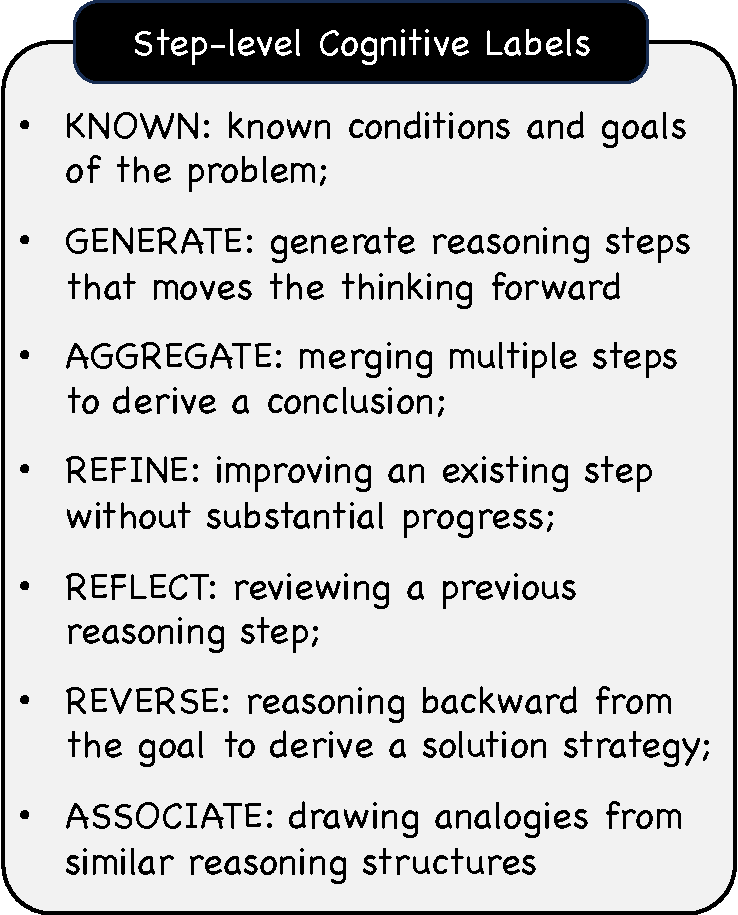
\includegraphics[width=0.86\linewidth]{Figures/labels.pdf}
    \caption{
    Step-level Cognitive Labels.
    }
    \label{fig:labels}
\end{figure}

\section{Graph-Structured Translation Prompt and Examples}
\label{app:translation}
\subsection{Graph-Structured Translation Prompt}
We design a unified prompt for graph-structured reasoning translation,
which specifies the node schema, thinking-mode tags, and dependency relations.
The prompt is shown in Figure~\ref{fig:prompt_grpah}.
The illustrative examples mentioned in the prompt are presented in the following subsections. The original Chain-of-Thought traces are generated using \texttt{Qwen3-Max-Preview}, which provides explicit thinking processes, and are subsequently translated into graph-structured representations using the \texttt{Qwen3-Max} model.

\subsection{Mathematical Examples}
We first present two mathematical examples that are originally included
in the graph-structured translation prompt.
The first example is designed to explicitly illustrate the use of
\emph{reverse thinking} and \emph{associative thinking}
(Figure~\ref{fig:math_example_reverse}).
The second example demonstrates another mathematical reasoning process
and is accompanied by a schematic visualization of its corresponding
reasoning graph, where nodes represent intermediate reasoning steps and
edges encode their dependency relations
(Figures~\ref{fig:math_example} and~\ref{fig:math_example_graph}).

\subsection{Code Generation Examples}
We include three code generation examples.
Each example corresponds to a representative question type of code generation task.

\begin{table*}[htbp]
    \centering
    \normalsize % 保持标准字号
    \caption{Ablation Study Results of Length-Reducing Rewards.}
    \label{tab:ablation_length}
    \renewcommand{\arraystretch}{1} % 保持行间距设置
    \begin{tabular}{lcccccc}
        \toprule
        \multirow{2}{*}{\textbf{Method}} & \multicolumn{2}{c}{\textbf{MATH500}} & \multicolumn{2}{c}{\textbf{AMC23}} & \multicolumn{2}{c}{\textbf{AIME24}} \\
        \cmidrule(lr){2-3} \cmidrule(lr){4-5} \cmidrule(lr){6-7}
        & \textbf{Acc.} & \textbf{Length} & \textbf{Acc.} & \textbf{Length} & \textbf{Acc.} & \textbf{Length} \\
        \midrule
        PASC-GRPO                & 91.20 & 1260 & 82.50 & 1960 & 46.67 & 7040 \\
        w/o Connectivity         & 91.35 & 1850 & 81.55 & 2140 & 45.10 & 11200 \\
        w/o Conn. \& ERS Ratio & 90.52 & 1920 & 79.12 & 2483 & 43.25 & 22500 \\
        \bottomrule
    \end{tabular}
\end{table*}

% \begin{table}[htbp]
%     \centering
%     \small
%     \caption{Ablation Study of Length-Reducing Rewards. Only reasoning length (number of nodes) is reported.}
%     \label{tab:ablation_length_single}
%     \renewcommand{\arraystretch}{1} % 行间距
%     \begin{tabular}{lccc}
%         \toprule
%         \textbf{Method} & \textbf{MATH500} & \textbf{AMC23} & \textbf{AIME24} \\
%         \midrule
%         PASC-GRPO                & 1260  & 1960  & 7040  \\
%         w/o Connectivity         & 1850  & 2840  & 11200 \\
%         w/o Conn. \& ERS Entropy & 3120  & 5400  & 22500 \\
%         \bottomrule
%     \end{tabular}
% \end{table}


\begin{itemize}
    \item \textbf{Code Completion (Complete).}
    This type simulates the automatic code completion scenario in
    integrated development environments (IDEs).
    The model is provided with a function signature and a docstring as context
    and is required to generate the remaining function body.
    This task reflects the core capabilities of base code models such as
    Codex and StarCoder, primarily evaluating syntactic correctness and
    context-aware continuation, as exemplified by benchmarks like HumanEval
    (see Figure~\ref{fig:code_complete}).

    \item \textbf{Instruction Following (Instruct).}
    Also referred to as instruction-based or conversational code generation,
    this paradigm evaluates a model's alignment with human intent.
    The input consists of a natural language description of a programming task,
    and the model must generate a corresponding functional implementation.
    This setting is the dominant evaluation protocol for instruction-tuned
    models such as GPT-4 and DeepSeek-Coder-Instruct, emphasizing the
    translation of natural language semantics into executable logic
    (see Figure~\ref{fig:code_instruct}).

    \item \textbf{Competitive Programming (Online Judge).}
    This type emulates algorithmic contest environments such as ACM-style
    competitions or online judges (e.g., LeetCode).
    Unlike instruction-following tasks that generate a single function,
    competitive programming requires the model to produce a complete script
    that handles standard input and output streams.
    As a result, this paradigm is widely regarded as the most challenging
    form of code generation, demanding advanced algorithmic reasoning as well
    as robust handling of input parsing, output formatting, and edge cases
    (see Figure~\ref{fig:code_cp}).
\end{itemize}


\section{Graphical CoT Verification and Refinement Prompt}
\label{app:verify}

This appendix presents the prompt for graphical Chain-of-Thought (CoT)
verification and refinement, which is shown in Figure~\ref{fig:prompt_verify}. All verification and refinement results are generated using the \texttt{Qwen3-Max} model.

\section{Training Data}
\label{app:training_data}

\subsection{Supervised Fine-Tuning (SFT) Data}
\begin{itemize}
    \item \textbf{Math Reasoning}.
    We use the full 40.3k samples from the DeepScaleR dataset.
    
    \item \textbf{Code Generation}.
    We curate 12k samples from the KodCode-V1-SFT-R1 subset,
    balancing task difficulty
    ($Easy:Middle:Hard = 4:3:3$)
    and task types
    ($Complete:Instruct:Online\_Judge = 4.5:4.5:1$).
\end{itemize}

\subsection{Reinforcement Learning (RL) Data}
\begin{itemize}
    \item \textbf{Math Reasoning}.
    We sample 5,000 problems from the DeepScaleR dataset.
    Problems are attempted four times by Qwen3-8B and stratified by difficulty
    based on success count.
    Problems failed in all attempts are discarded, followed by stratified
    sampling with a ratio of $1:1:1.5:1.5$.
    
    \item \textbf{Code Generation}.
    We directly employ the KodCode-Light-RL-10K subset.
\end{itemize}

\subsection{Data Leakage Check}
\label{app:data_leakage}

To prevent potential data leakage, we first collected all evaluation test sets relevant to our tasks.  
After selecting the training data for both supervised fine-tuning and reinforcement learning, we cross-checked each training sample against these test sets.  
Any overlapping instances would have been removed.  
Our inspection confirmed that the training sets contain no examples from the test sets, ensuring a clean separation between training and evaluation data.


\section{Ablation Study Details}
\label{app:ablation}

Table~\ref{tab:ablation_length} reports the detailed ablation results of
the proposed length-reducing rewards across multiple math reasoning benchmarks.
We progressively remove the connectivity reward and ERS information ratio,
to examine their individual contributions.
The results show that removing these components leads to a substantial
increase in reasoning length and a consistent degradation in accuracy,
especially on more challenging benchmarks such as AIME24,
highlighting their importance in controlling reasoning efficiency
without sacrificing correctness.

\begin{figure*}[t]
    \centering
    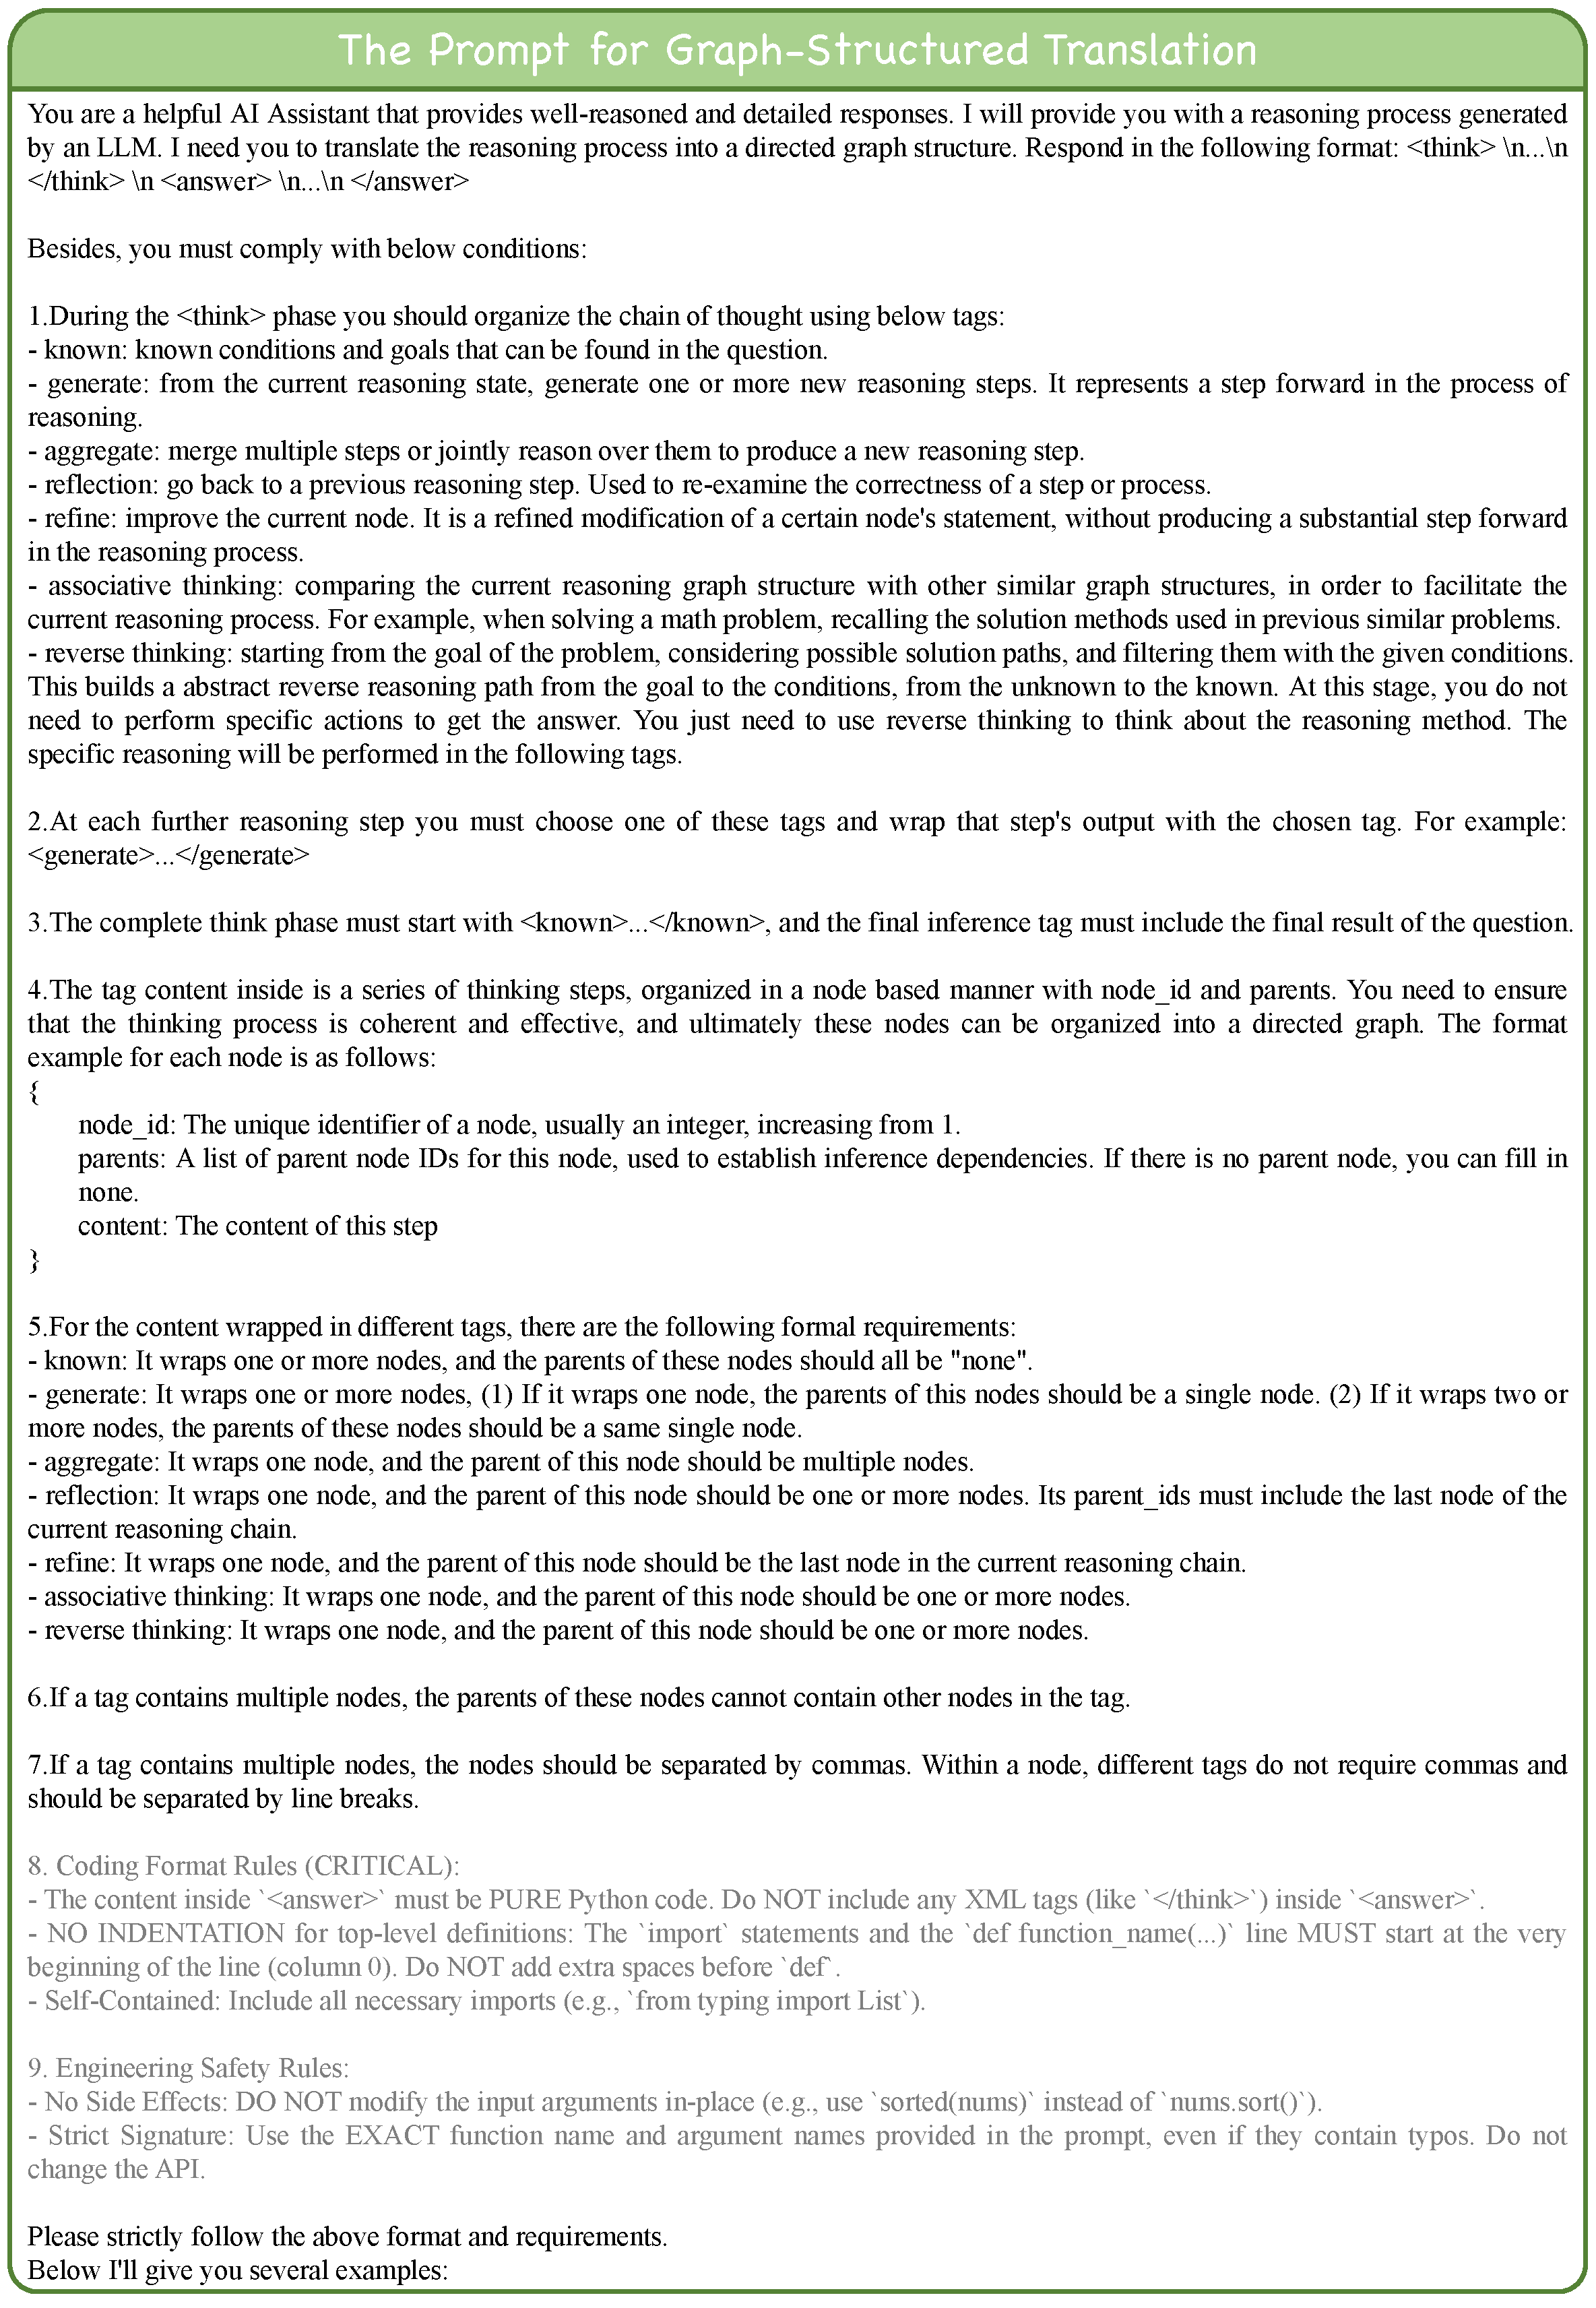
\includegraphics[width=\linewidth]{Figures/The_Prompt_for_Graph-Structured_Translation.pdf}
    \caption{
    The prompt template for ``Graph-Structured Translation''. Criteria 8 and 9 are specifically added to accommodate code generation task.
    }
    \label{fig:prompt_grpah}
\end{figure*}

\begin{figure*}[htbp]
    \centering
    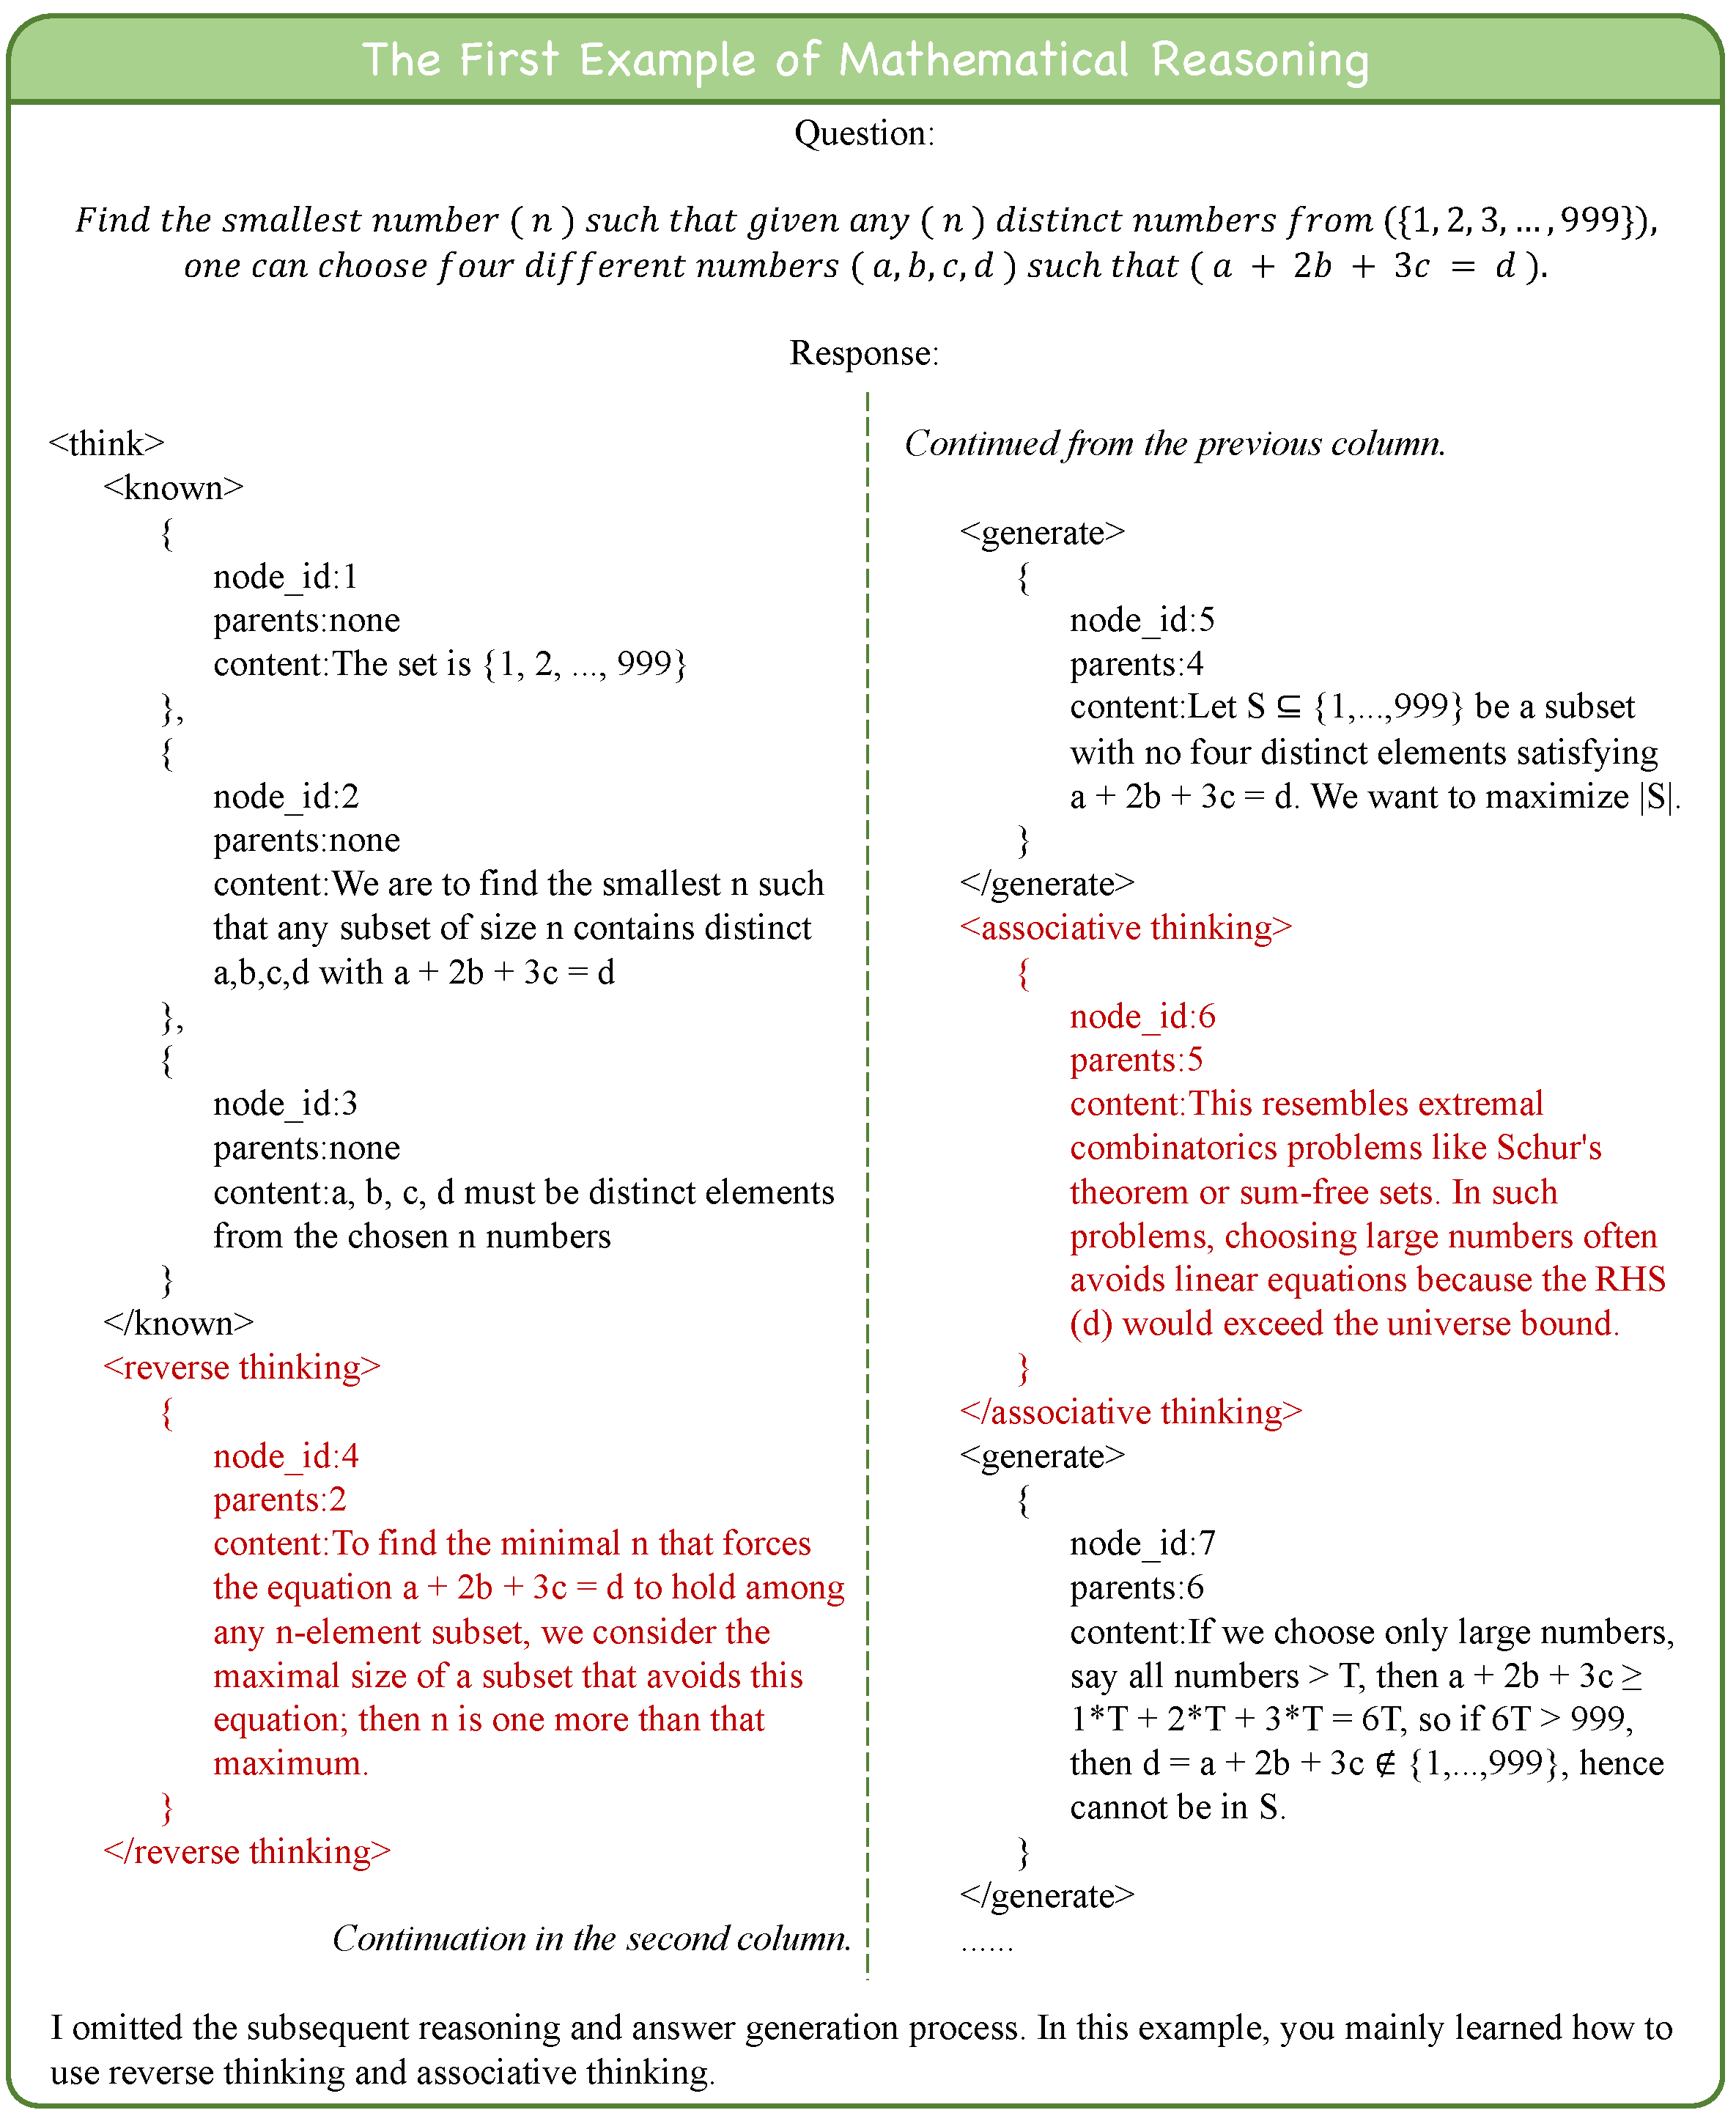
\includegraphics[width=\textwidth]{Figures/math_example_1.pdf}
    \caption{A mathematical example illustrating reverse and associative thinking.}
    \label{fig:math_example_reverse}
\end{figure*}

\begin{figure*}[htbp]
    \centering
    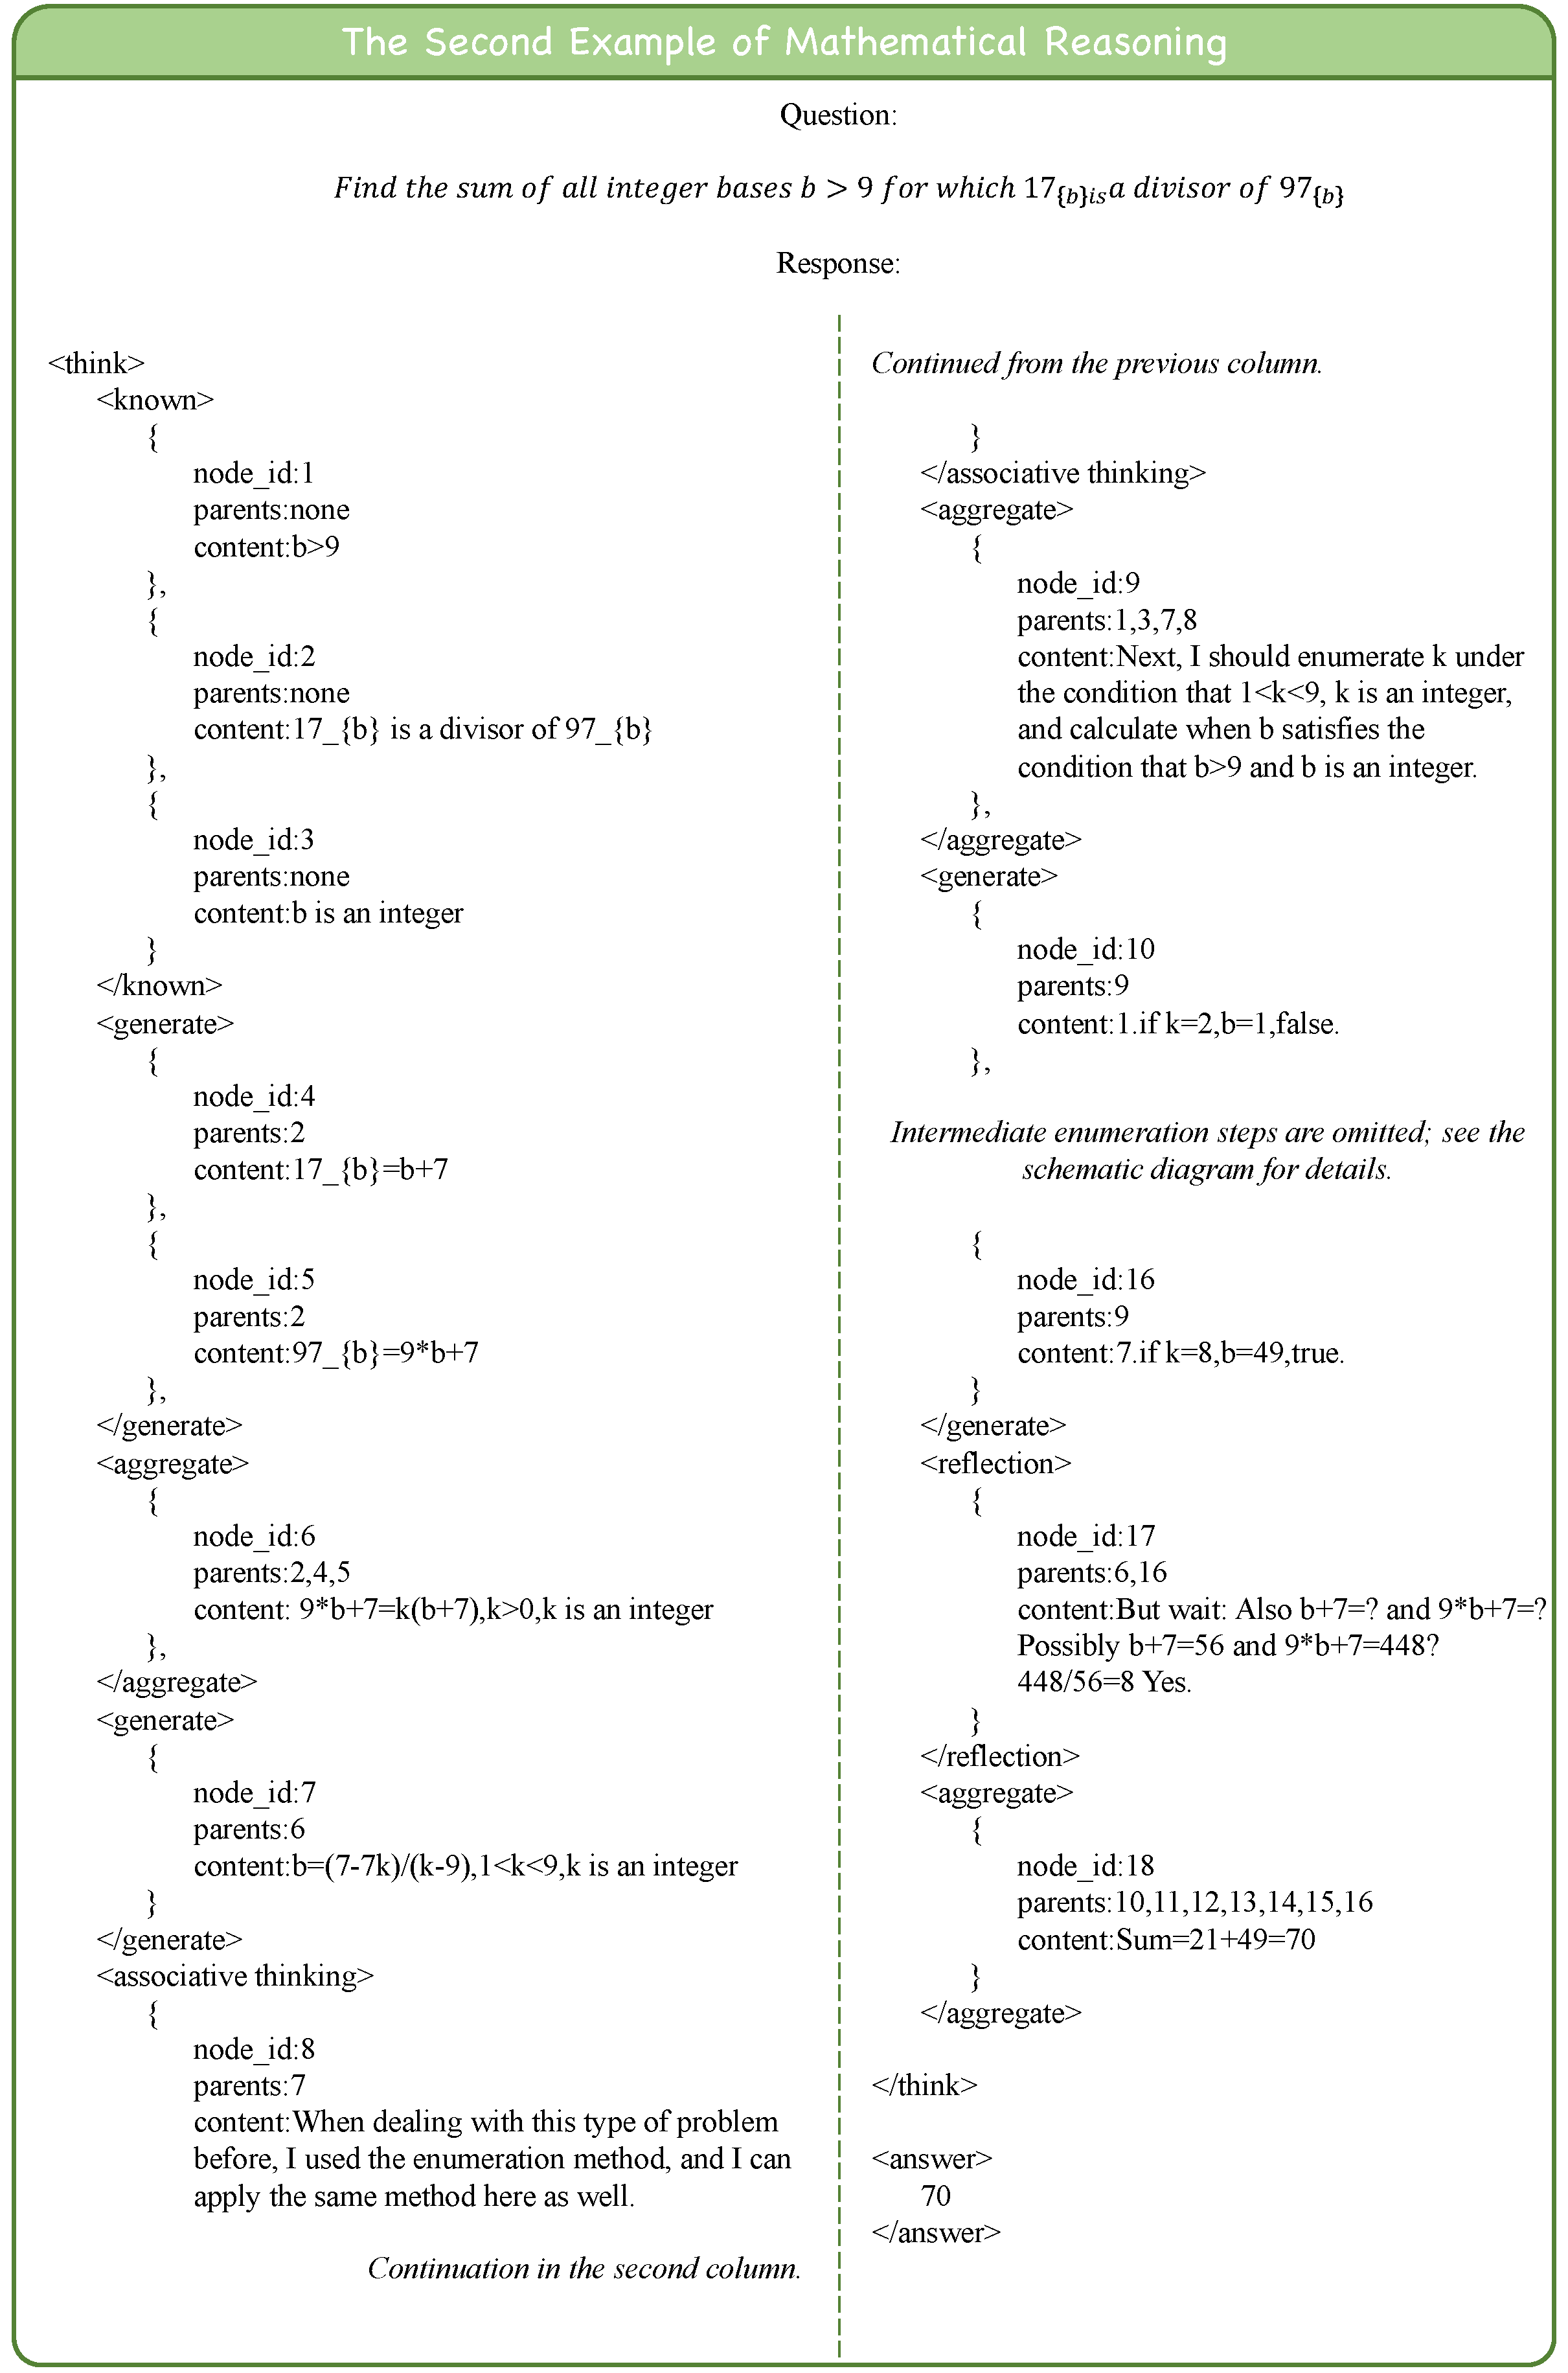
\includegraphics[width=\textwidth]{Figures/math_example_2.pdf}
    \caption{A mathematical example in graph-structured format.}
    \label{fig:math_example}
\end{figure*}

\begin{figure*}[htbp]
    \centering
    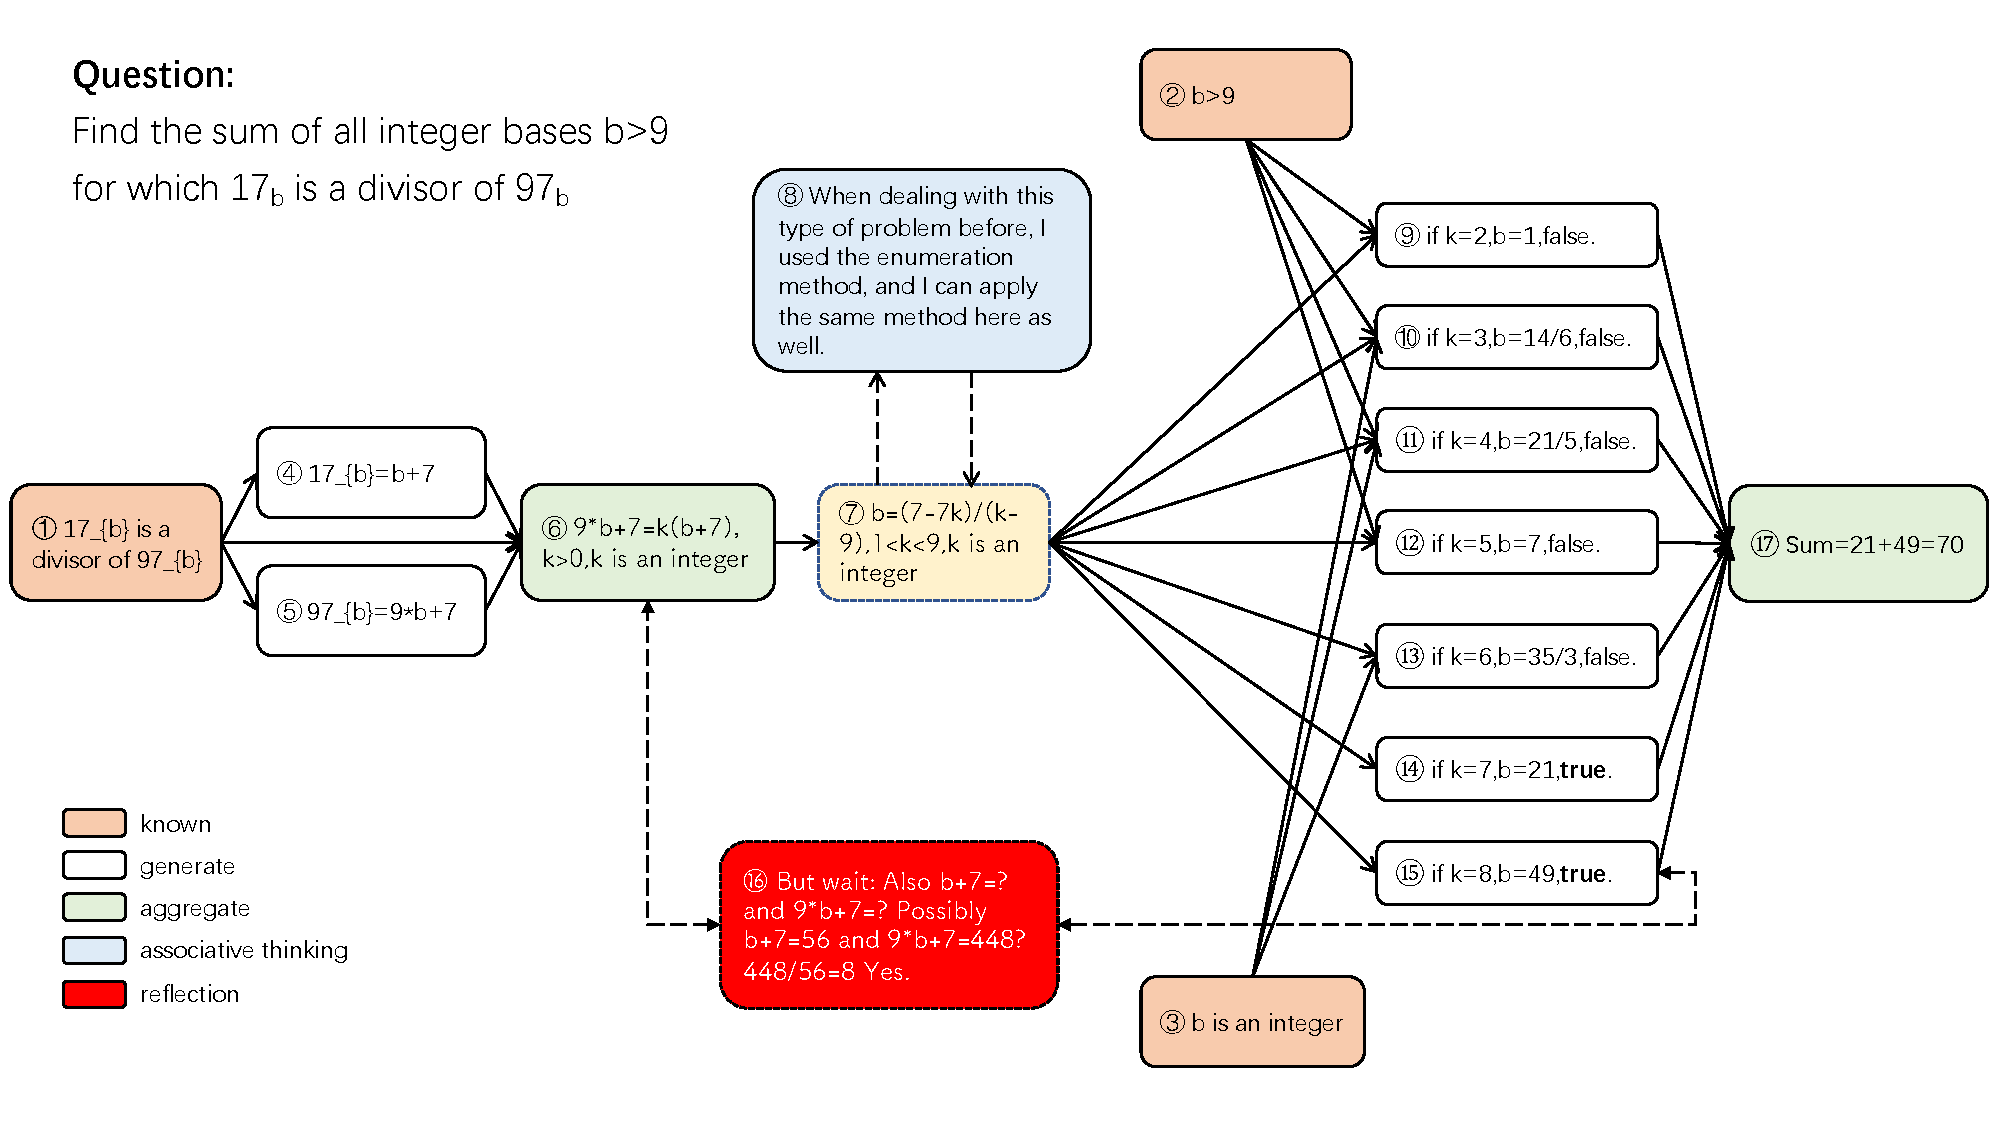
\includegraphics[width=\linewidth]{Figures/example.pdf}
    \caption{Graph visualization of the mathematical example.}
    \label{fig:math_example_graph}
\end{figure*}

\begin{figure*}[htbp]
    \centering
    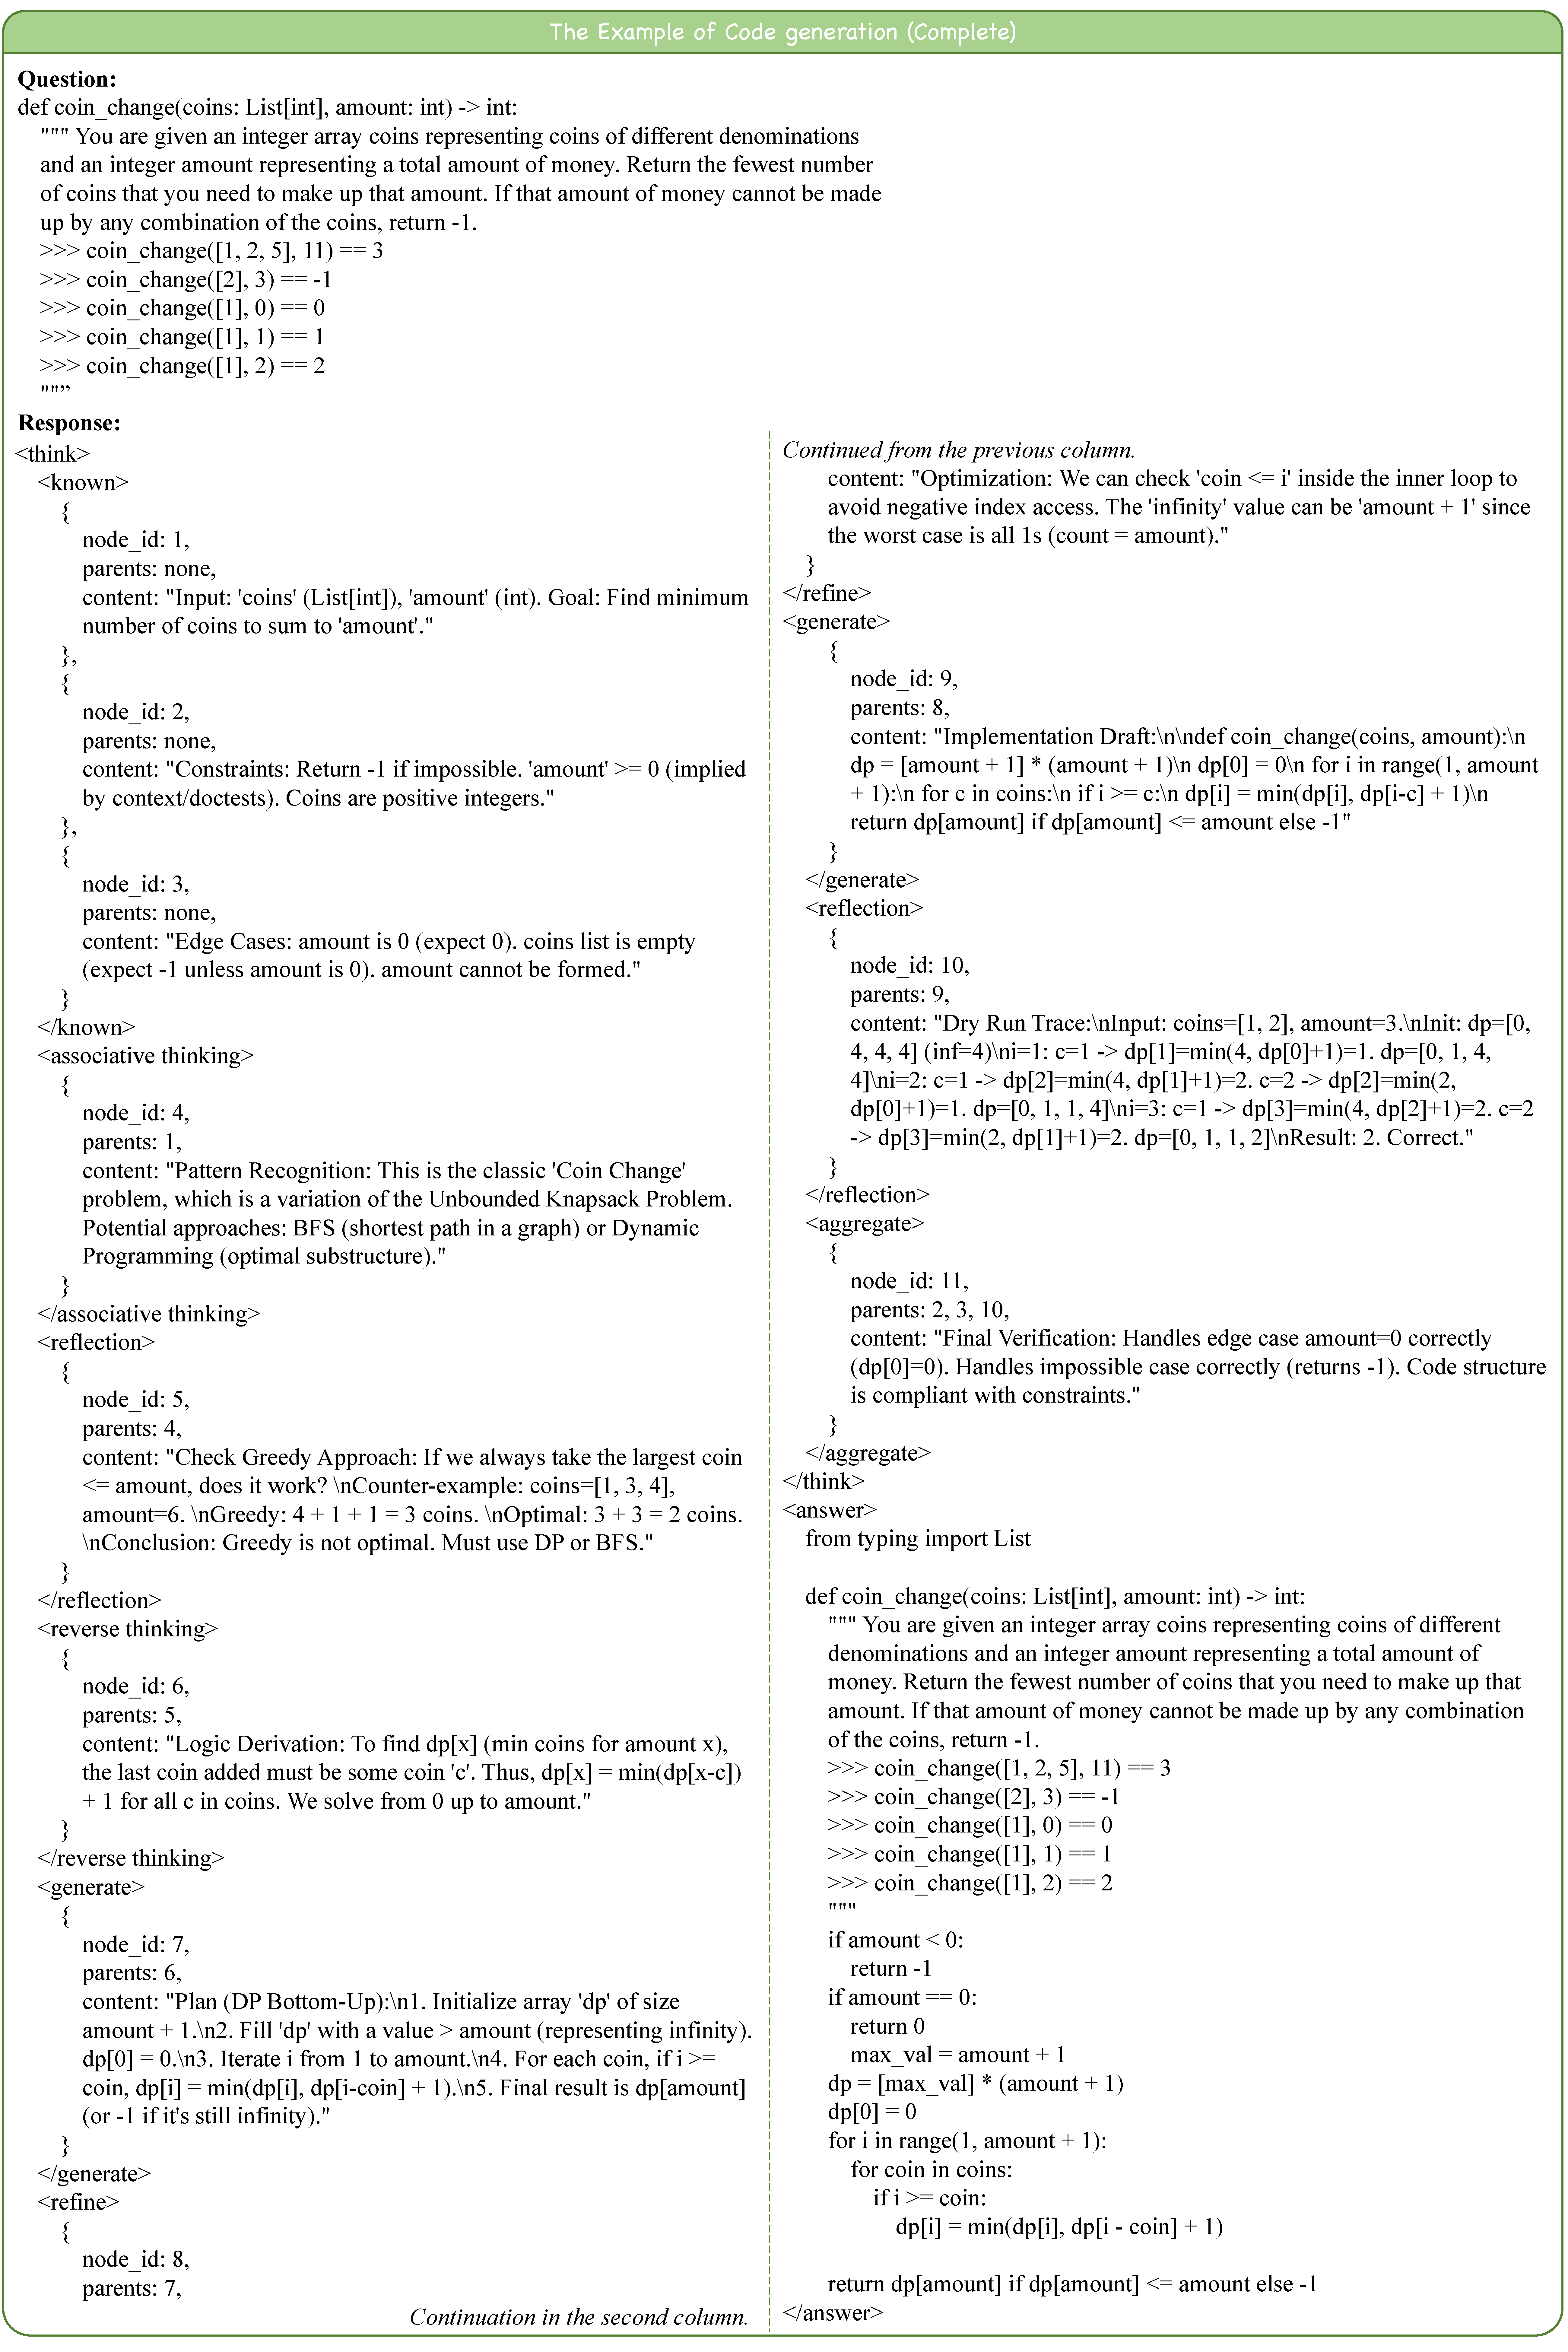
\includegraphics[width=\textwidth]{Figures/code_example_1.pdf}
    \caption{A code completion example.}
    \label{fig:code_complete}
\end{figure*}

\begin{figure*}[htbp]
    \centering
    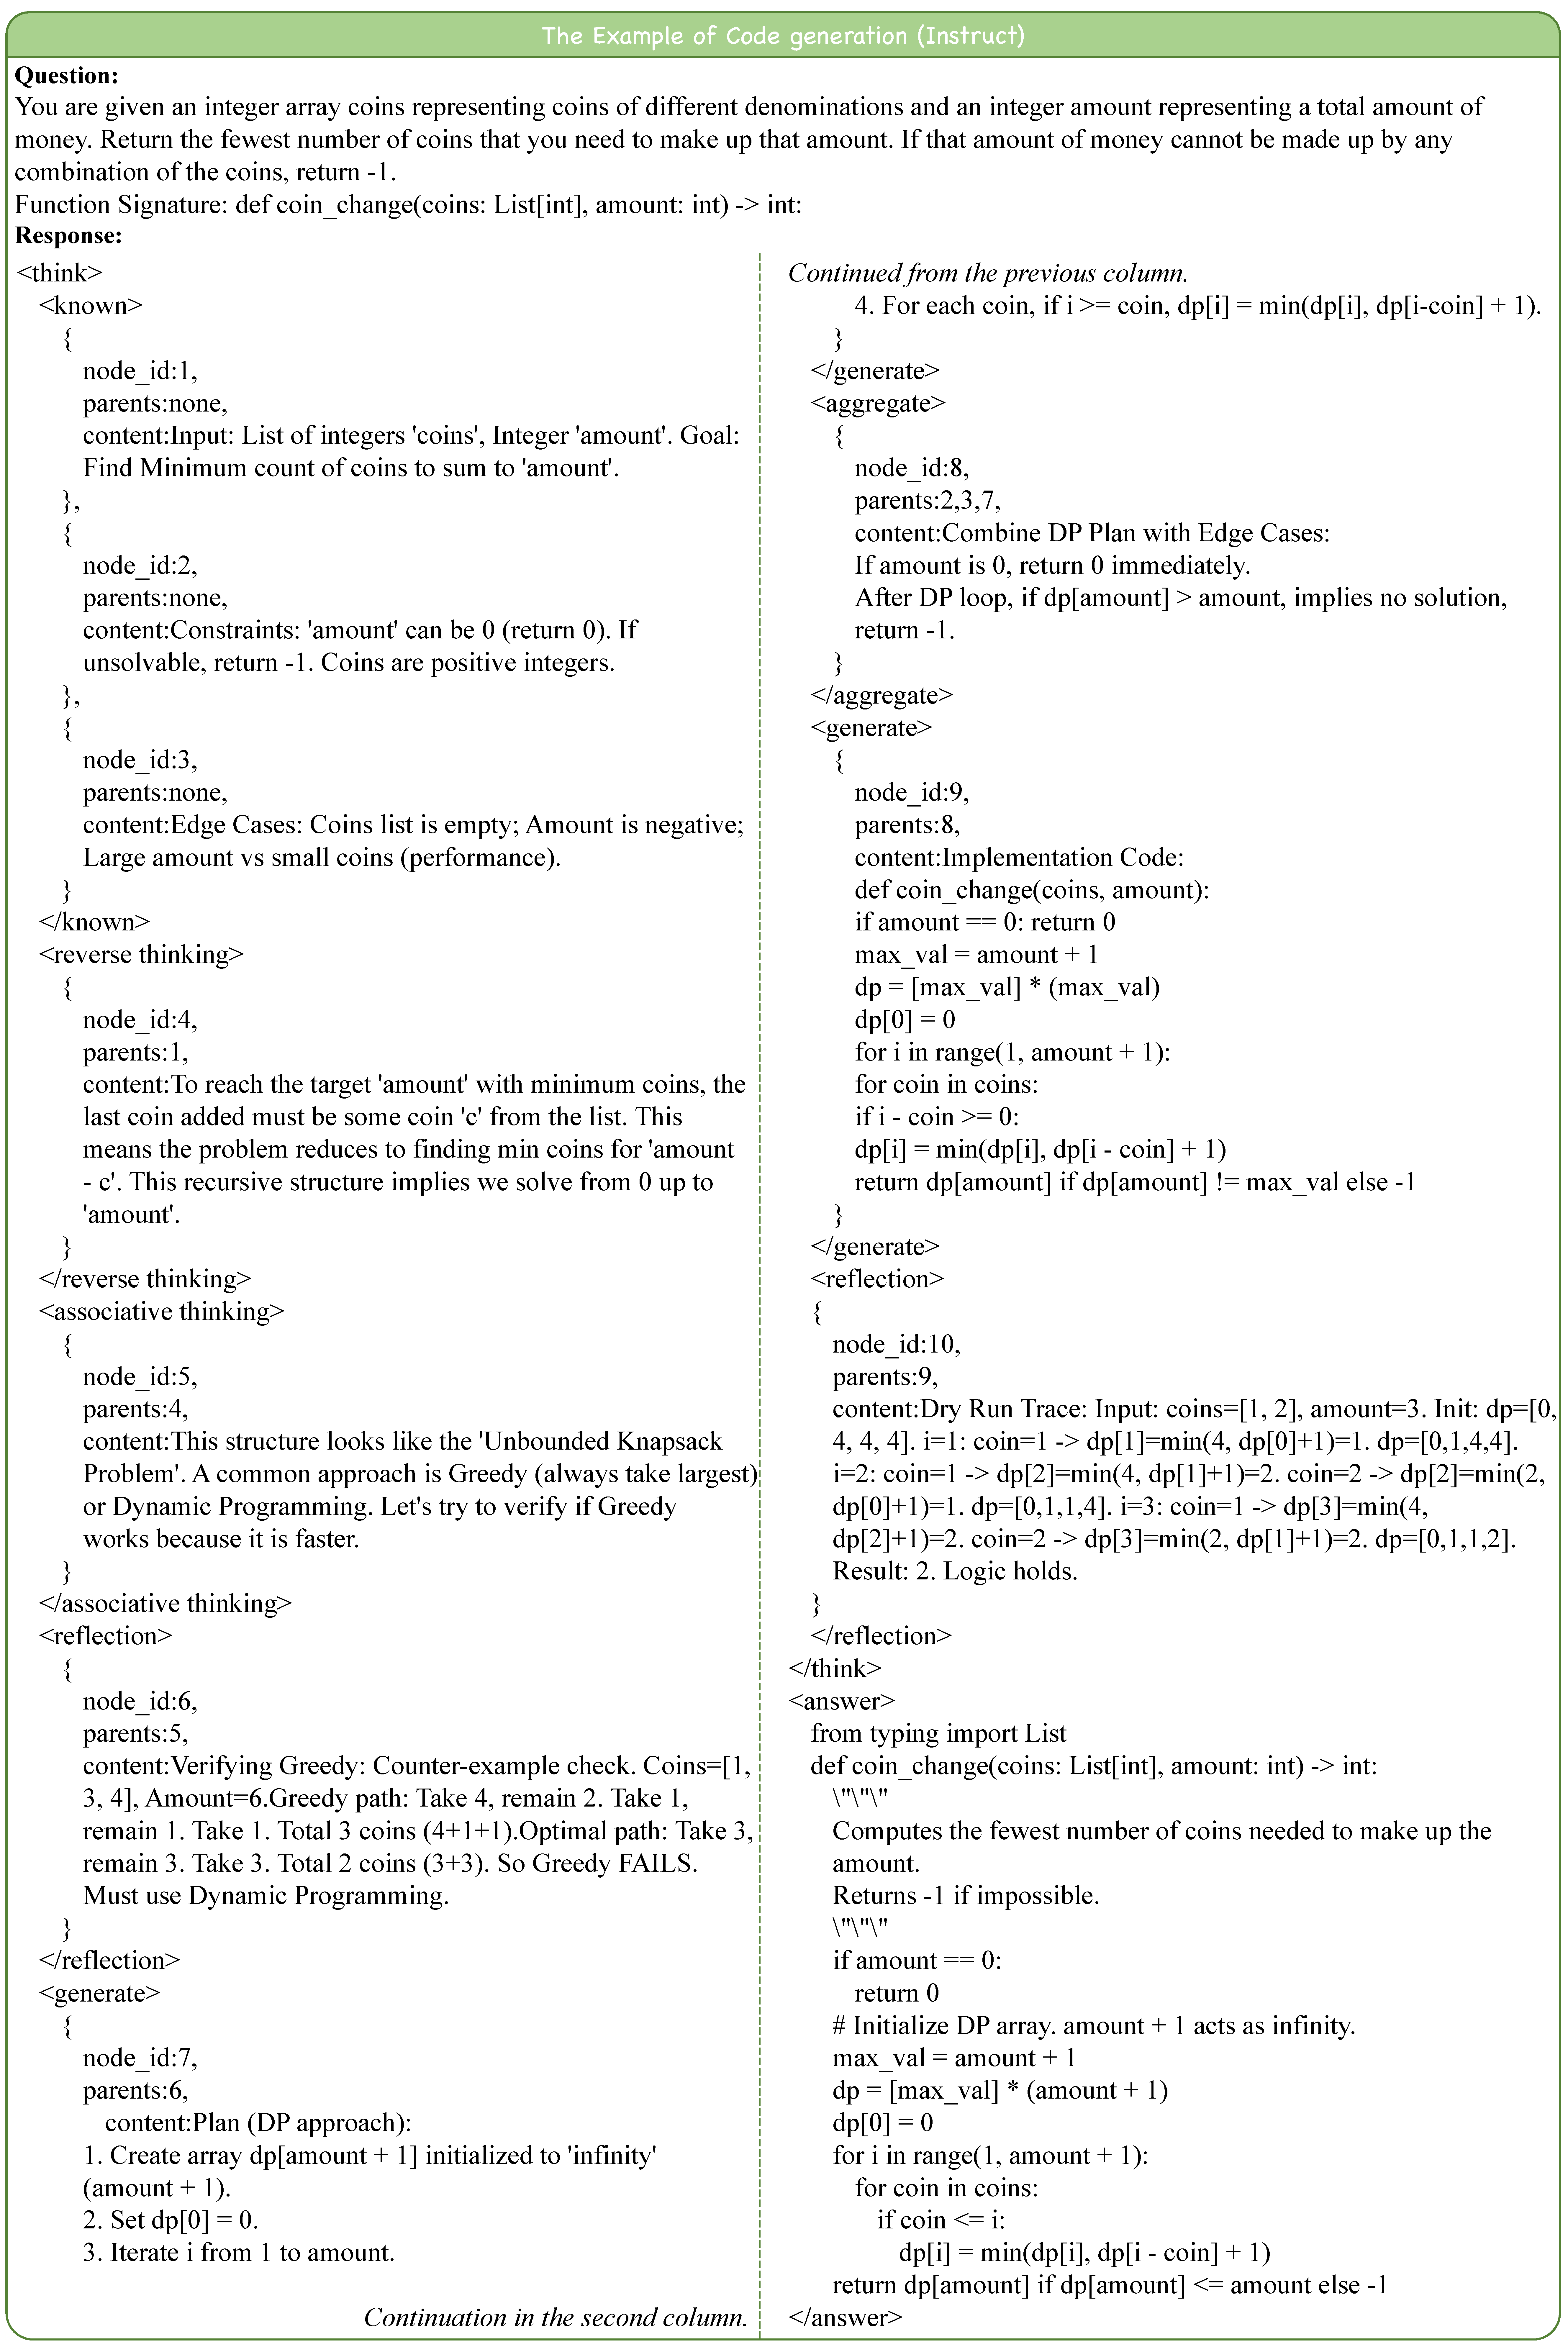
\includegraphics[width=\textwidth]{Figures/code_example_3.pdf}
    \caption{An instruction-following code generation example.}
    \label{fig:code_instruct}
\end{figure*}

\begin{figure*}[htbp]
    \centering
    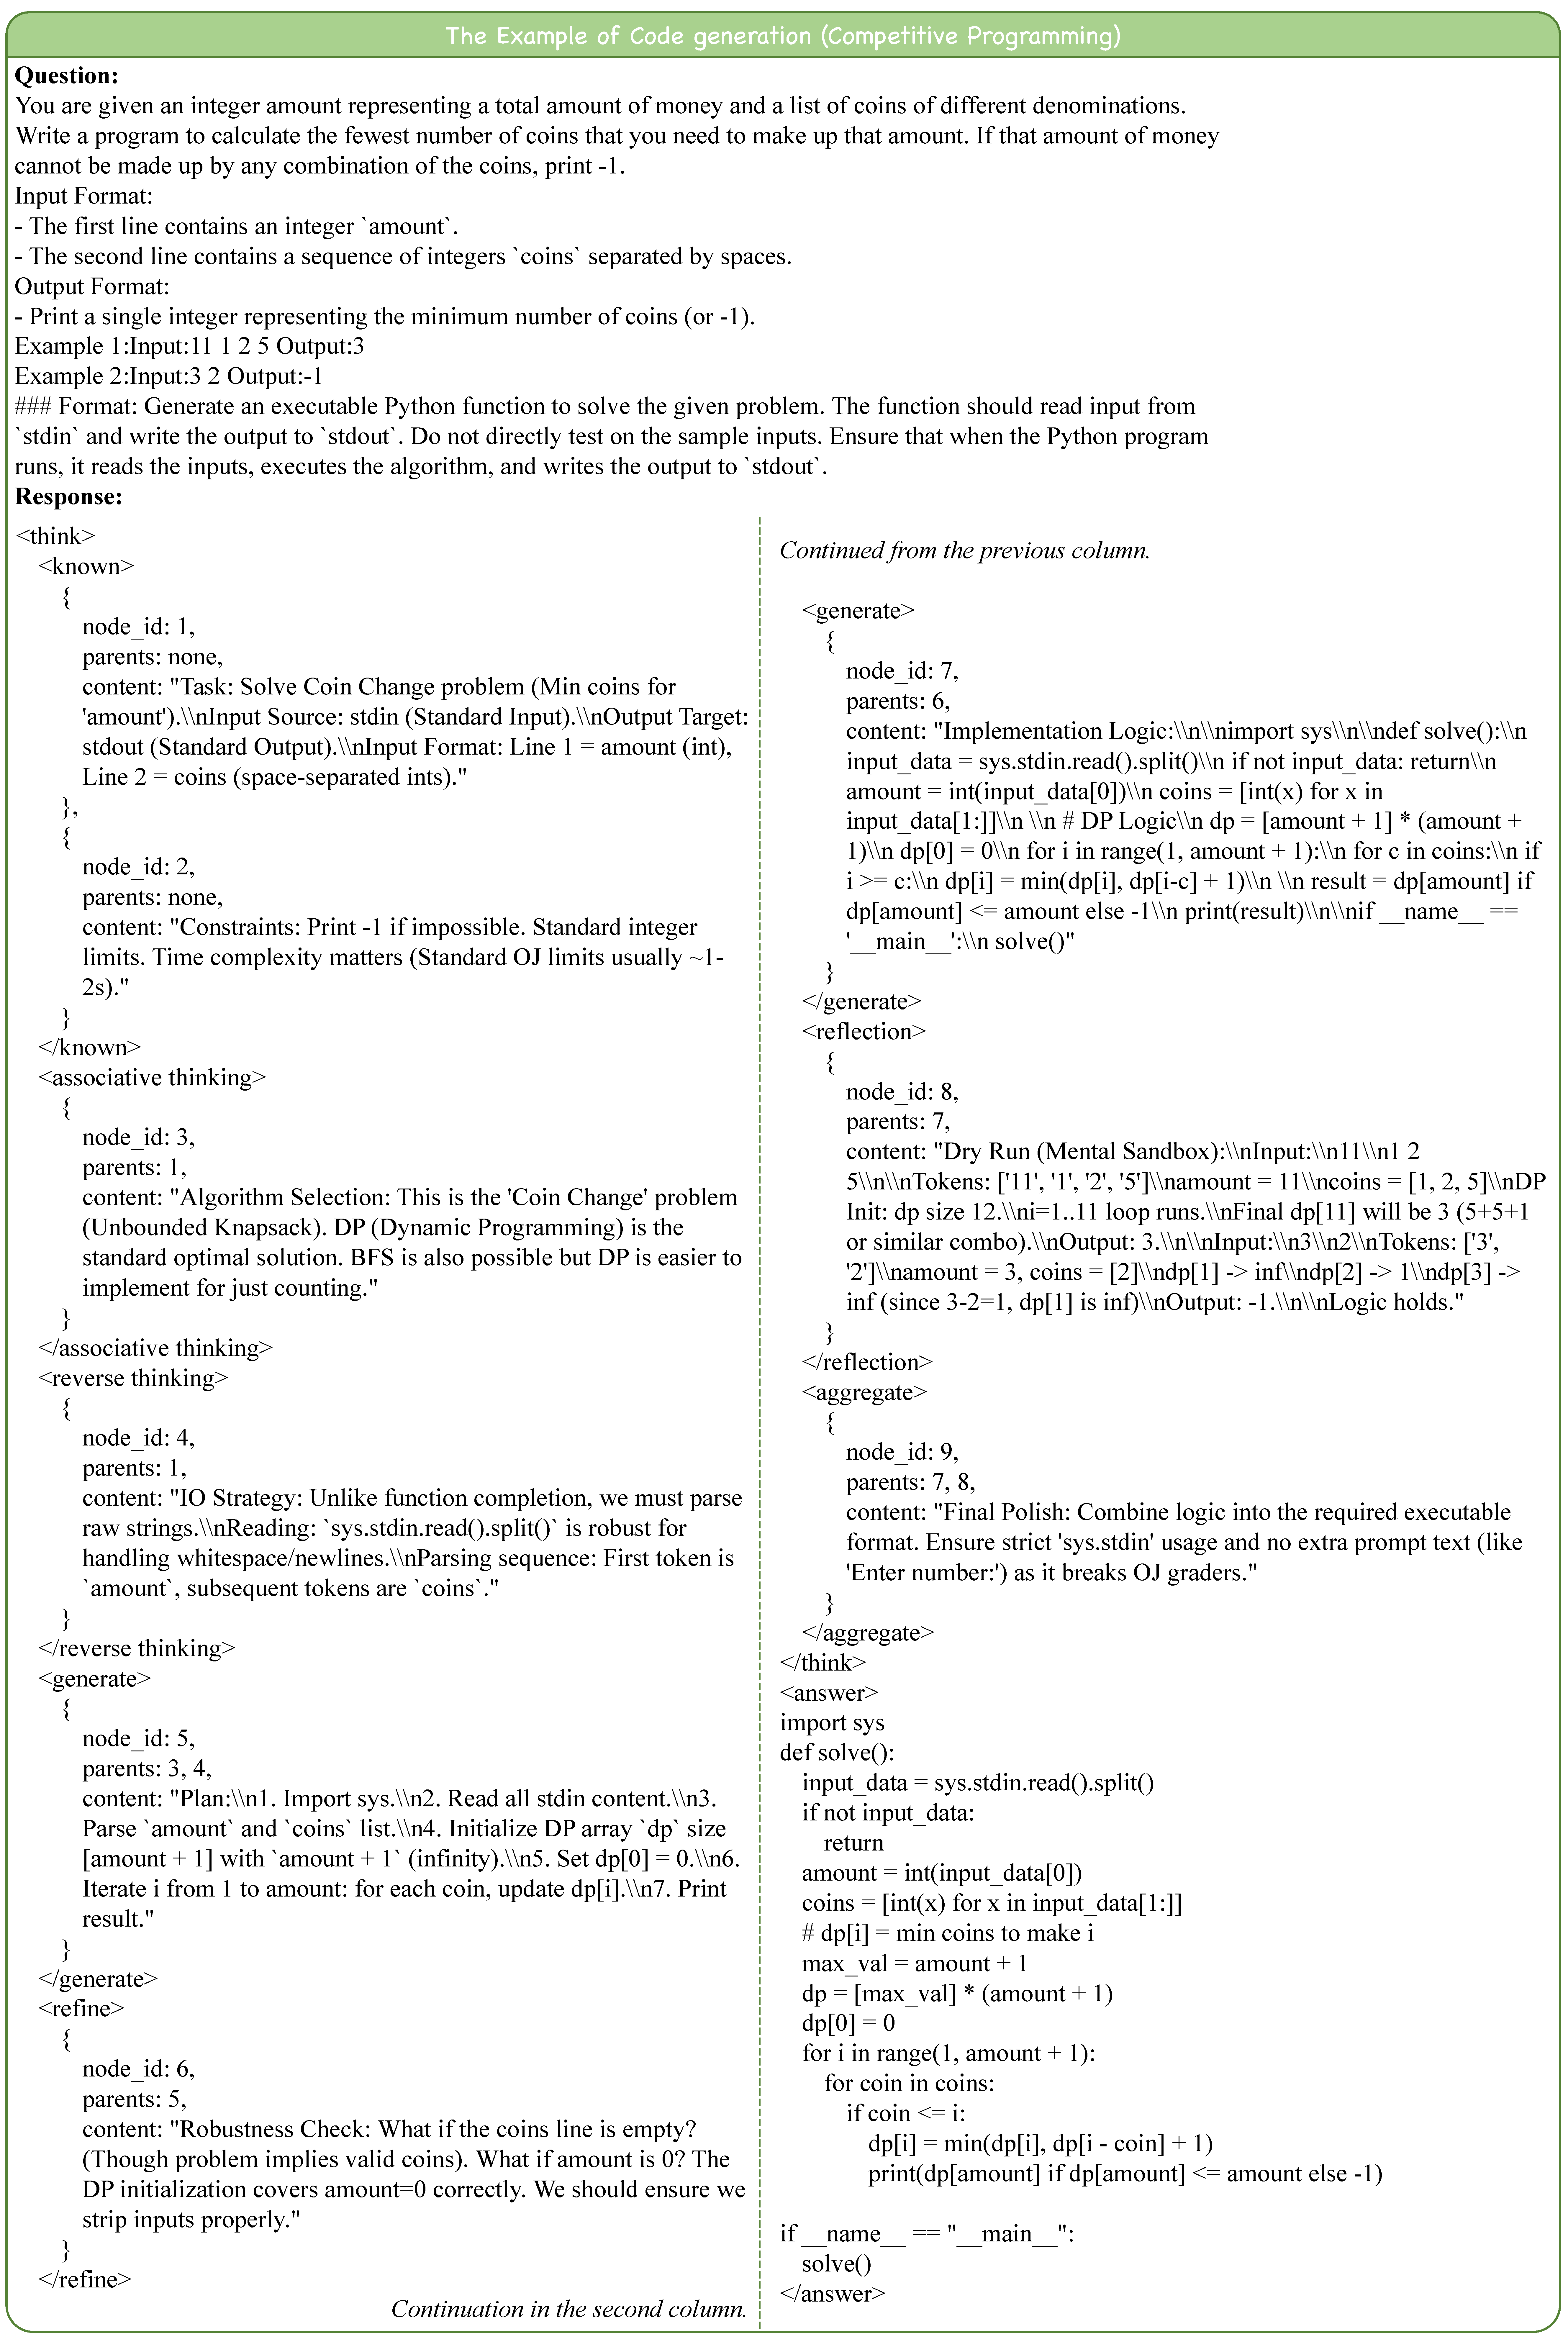
\includegraphics[width=\textwidth]{Figures/code_example_2.pdf}
    \caption{A competitive programming code generation example.}
    \label{fig:code_cp}
\end{figure*}

\begin{figure*}[htbp]
    \centering
    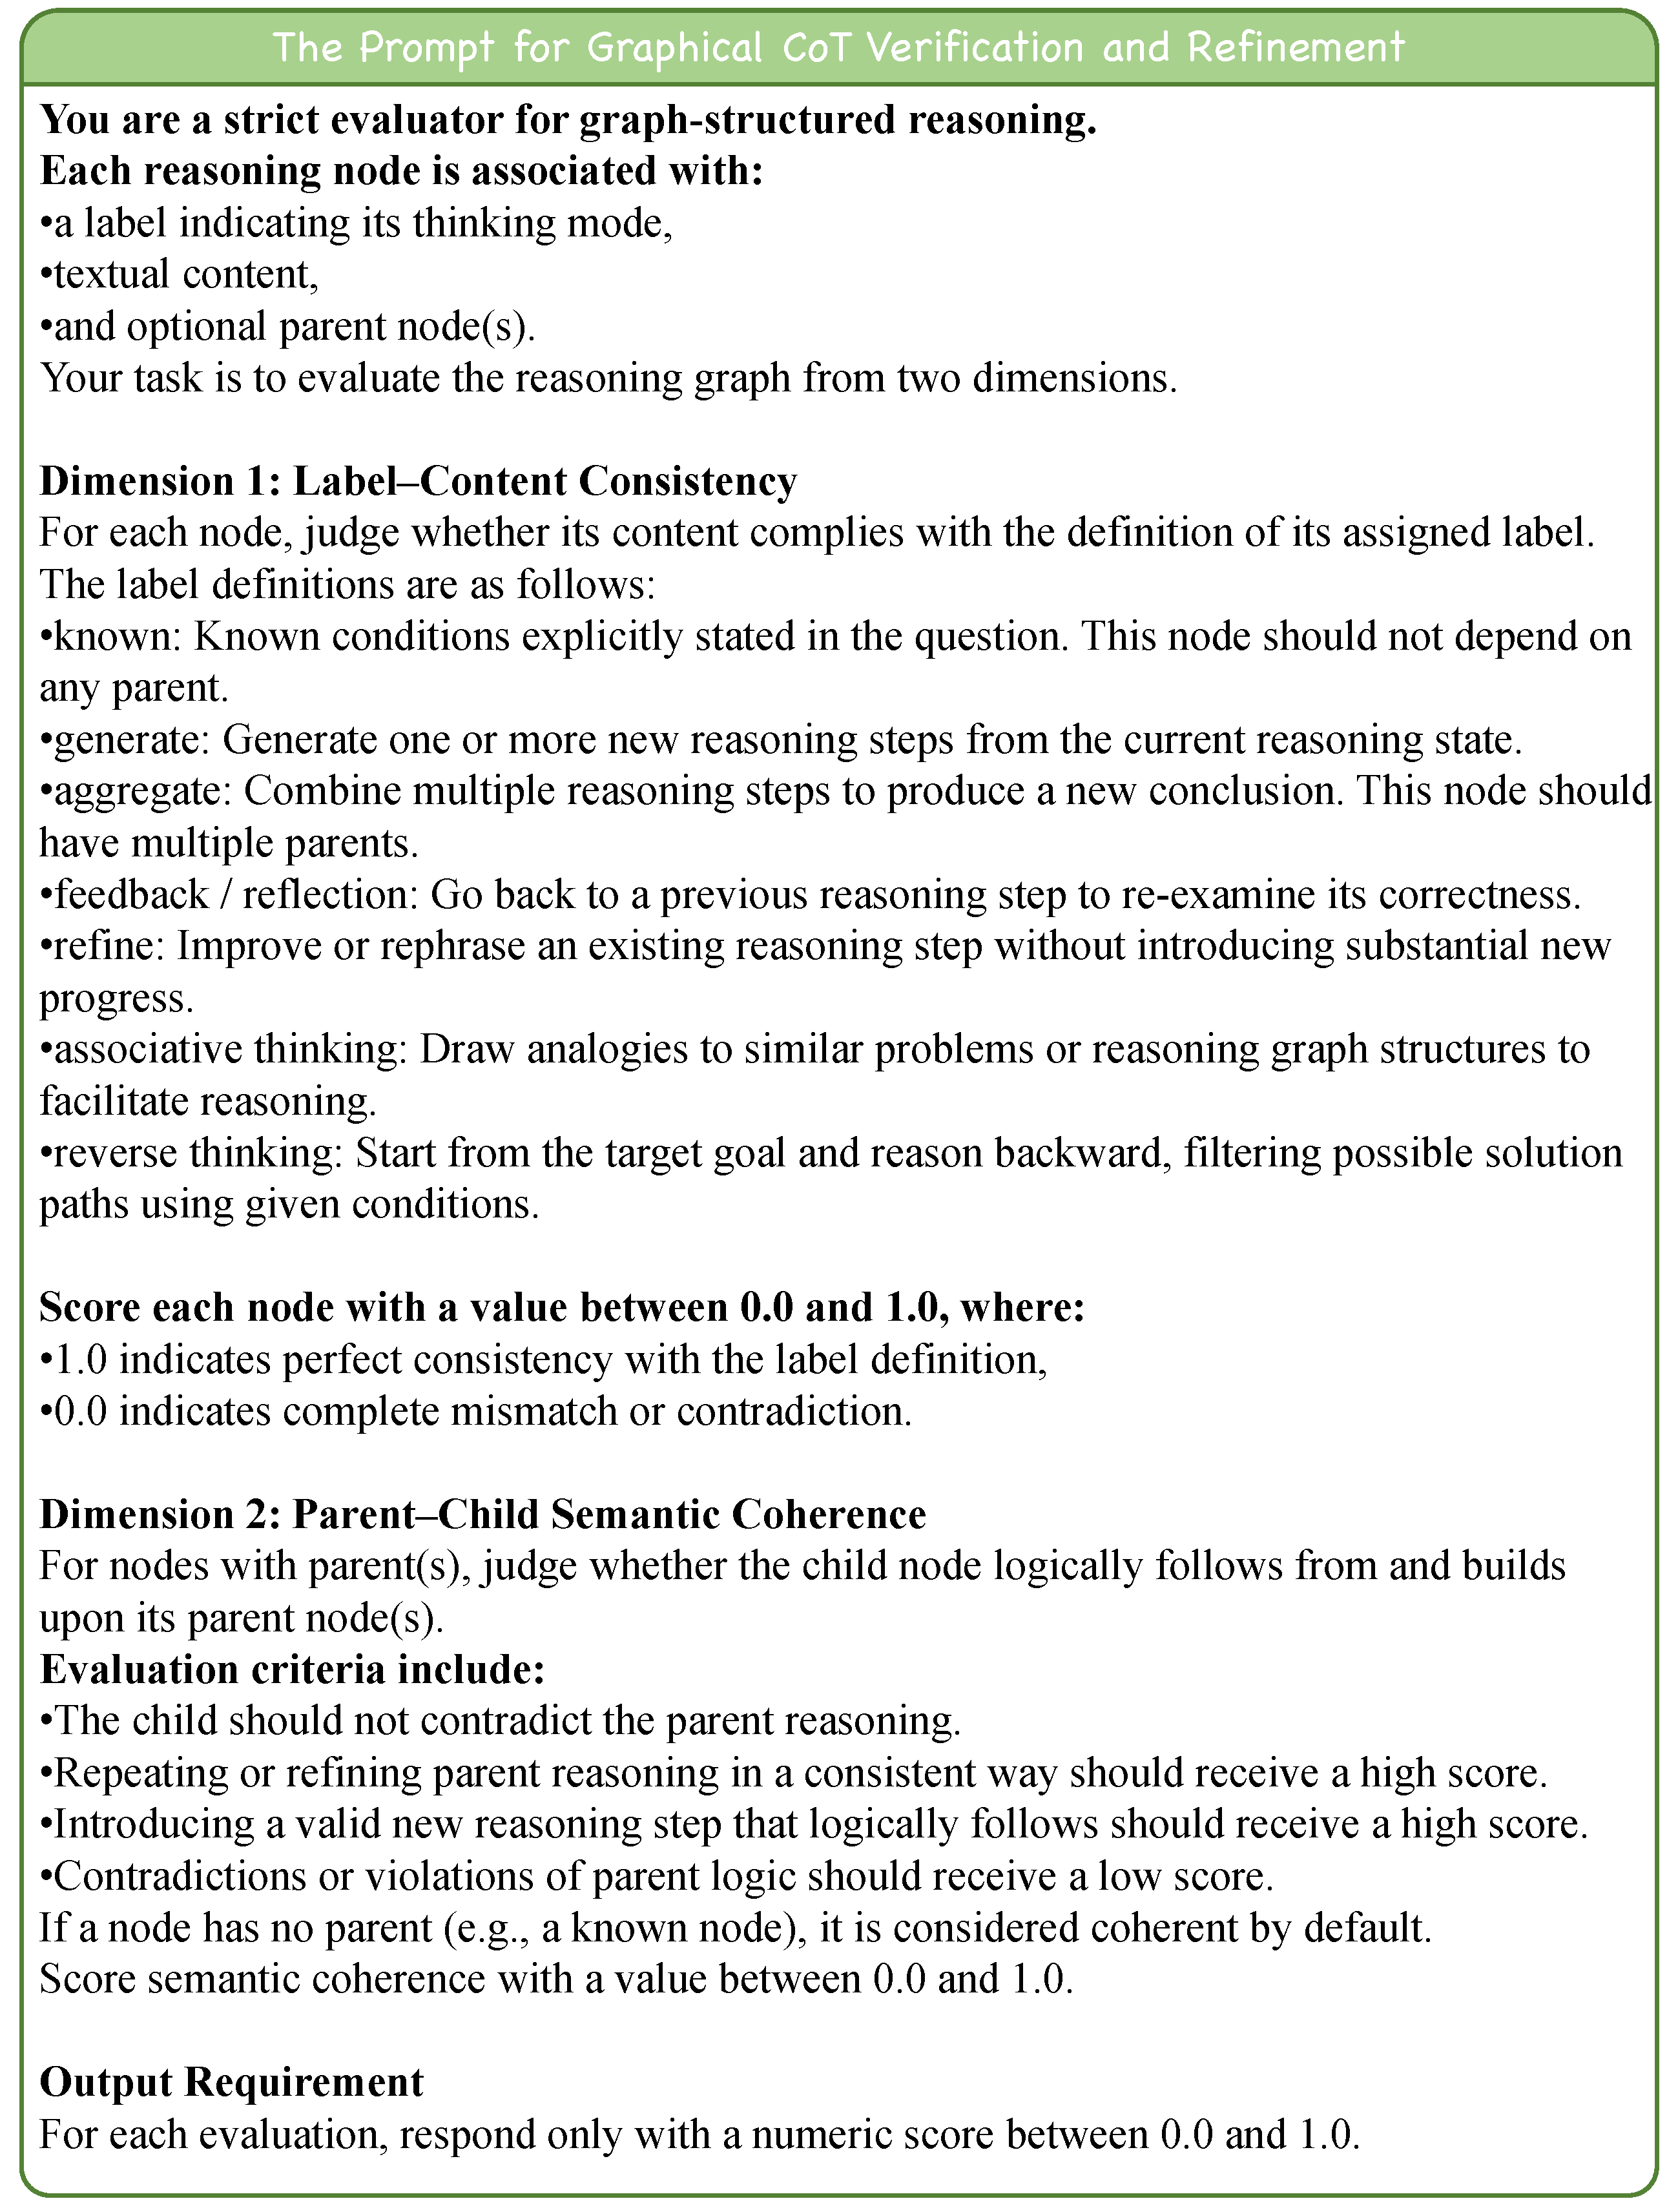
\includegraphics[width=\linewidth]{Figures/The_Prompt_for_Graphical_CoT_Verification_and_Refinement.pdf}
    \caption{Prompt for ``Graphical CoT Verification and Refinement''.}
    \label{fig:prompt_verify}
\end{figure*}

